\chapter{Proposta}


A adoção de padrões é uma premissa básica para o desenvolvimento de software, pois ao trabalhar com variações dentro de uma organização, a tendência é gerar confusão. Assim, o objetivo deste trabalho é projetar e implementar um módulo padrão de permissões de acesso, de modo que o mesmo possa ser utilizado por diferentes plataformas, como desktop, Web e mobile, eliminando assim este módulo do desenvolvimento de um software e utilizando o trabalho proposto como um SaaS provedor das permissões do software cliente a ser desenvolvido.


É comum encontrar frameworks de desenvolvimento de software que automatizam a geração de esquemas de configuração de módulos com perfis de acesso. Entretanto, apesar de ser um facilitador, tal política pode se tornar confusa em algus cenários, a exemplo de uma empresa que trabalha com sistemas sob encomenda, onde o cliente pode até mesmo determinar a linguagem ou framework de desenvolvimento. Nesse caso, a empresa teria que treinar os seus colaboradores a configurar os softwares para cada uma das ferramentas utilizadas, o que potencialmente ocasionaria dificuldades de entendimento comum.


Diante da possibilidade de manter a configuração dos sistemas de uma mesma instituição com diferentes módulos de permissão, seria ideal que todos os sistemas de software por ela desenvolvidos utilizassem um mesmo módulo de configuração de persmissão de acesso, para que esta parte comum, presente na maioria dos softwares, fosse padronizada.


O capítulo corrente é composto por três seções. A seção \ref{sec:arquitetura} trata da arquitetura do software proposto, contendo informações sobre as tecnologias utilizadas, diagramas UML e os requisitos do sistema. A seção \ref{sec:processo} demonstra o fluxo do processo empregado na aplicação desenvolvida e por fim, a seção \ref{sec:novidades} trada do que há de novo sob o ponto de vista tecnológico.

\section{Arquitetura da aplicação}\label{sec:arquitetura}


A aplicação desenvolvida neste trabalho foi arquitetada com o modelo SPA(Single page application) utilizando o AngularJs. Tal arquitetura se tornou tão popular quanto o famoso MVC (Model-View-Controller), e é bastante utilizada no desenvolvimento de aplicações web e mobile. Em linhas gerais, o conceito SPA tende a reduzir a necessidade de se implementar código server-side, e sim potencializar as ações em client-side. Assim, boa parte da aplicação passa a ser processada no cliente (dentro do navegador Web).


%\begin{figure}
%	\label{fig:spa}
%	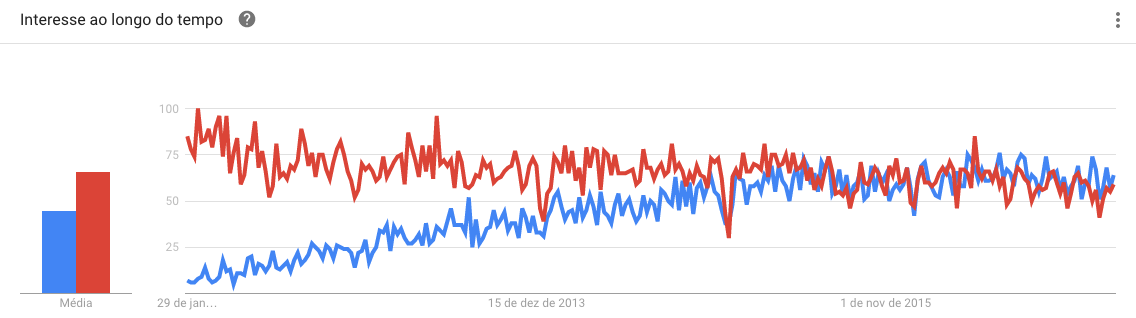
\includegraphics[width=1\textwidth]{img/spa-mvc}
%	\caption{Gráfico do Google Trends exibindo comparação entre as pesquisas por SPA e MVC}
%\end{figure}
não faça simplesmente copiar de um blog. tente ir além, e prover fundamentação contida em livros-texto da área.
um sugestão: capture as ideias do autor do blog, porém complemente-as com outras fontes, assegurando-se de que o que o autor do blog descreve de fato faz sentido na prática

Algumas vantagens da SPA:
\begin{itemize}

\item Partilha de processamento do software, visto que a aplicação consome uma API REST(back-end) e deve tratar os dados para a exibição no front-end.
\item Com da partilha do processamento, tem-se uma menor codificação no servidor. Tal aspecto vem acompanhado com a distinção das responsabilidades, pois apenas o código do front-end trata de interface.
\item Diante das características de uma SPA, a "página única" tende a ser de fácil entendimento aos usuários, simplificando a navegação.
\item Como os acessos via dispositivos móveis é bastante significativo, há uma relevância no consumo de dados do software. Nesse quesito, uma SPA se comporta bem, devido à forma como consome os dados, com requisições AJAX que retornam JSON(Javascript object notation), que na realidade se resume apenas a dados estruturados.

\end{itemize}
O grande ator de app SPA é o código Javascript executado no cliente. Toda a aplicação pode ser construída simplesmente manipulando-se o DOM (Document Object Model) de forma nativa, ou com o uso de bibliotecas e frameworks Javascript que auxiliam na construção da aplicação. Estas bibliotecas e frameworks fornecem recursos para manipulação dinâmica do DOM, definição de templates de tela, chamadas assíncronas ao servidor, organização do código Javascript, etc. Dentres as diversas bibliotecas Javascript disponíveis, tem-se entre as mais difundidas: AngularJs\footnote{https://angularjs.org/}
, VueJs\footnote{https://vuejs.org/}, Backbone\footnote{http://backbonejs.org/}, ReactJs\footnote{https://facebook.github.io/react/}, Ember\footnote{http://emberjs.com/} e outras.


Do lado servidor, tem-se a execução das linguagens de programação tradicionais como PHP, ASP.NET, JSP e etc. Assim, de acordo com a necessidade, as mesmas provêem host de arquivos, acesso a banco de dados e tratam regras de negócios que não podem estar no código JavaScript do Front-end por questões de segurança. E é do lado servidor que a arquitetura REST (Representational State Transfer) pode ser utilizada, com o intuito de fornecer serviços do servidor à aplicação SPA proposta neste trabalho. É comum encontrar aplicação SPA utilizando serviços RESTFul. Uma aplicação no servidor que utiliza a arquitetura REST para prover serviços, então é chamada de RESTFul. Neste trabalho, foi desenvolvida uma aplicação RESTFul com o Framework PHP Laravel.


Ao construir uma aplicação utilizando a arquitetura REST, o protocolo HTTP é usado em sua essência, utilizando os métodos de requisição ao servidor: GET, POST, PUT e DELETE (os mais comuns), e cada um deles indica uma determinada ação a ser executada em um recurso específico do servidor.


A seguir, a subseção \ref{tecnologias} trata das tecnologias utilizadas no trabalho proposto, a \ref{diagramas} apresenta os diagramas UML do projeto e \ref{funcionalidades} trata das funcionalidades, formalizando os requisitos funcionais e não funcionais.


\subsection{Tecnologias utilizadas}\label{tecnologias}


\subsubsection{Laravel framework}


Laravel \footnote{https://laravel.com/} é um framework PHP livre e open-source para o desenvolvimento de sistemas Web que utilizam o padrão MVC (model, view, controller). O Laravel foi desenvolvido sob o MIT License, com o código-fonte hospedado no GitHub. Em Agosto de 2015, o Laravel já era o principal framework de projetos PHP no GitHub. 


Algumas características proeminentes do Laravel são sua sintaxe simples e concisa, um sistema modular com gerenciador de dependências dedicado, várias formas de acesso a banco de dados relacionais e vários utilitários indispensáveis no auxílio ao desenvolvimento e manutenção de sistemas. Diante da popularidade do framework, tem-se uma grande comunidade, o que facilita a aprendizgem pois facilmente encontra-se tutoriais. Inclusive além da documentação, o próprio Laravel disponibiliza o Laracasts \footnote{https://laracasts.com/}, que traz aos desenvolvedores uma série de vídeos ensinando as mais diversas funcionalidades encontradas no Laravel.


\subsubsection{AngularJs}


AngularJS é um framework JavaScript open-source, mantido por Google, que auxilia na execução de SPA. O framework lê o HTML que contém tags especiais do framework e então executa a diretiva na qual esta tag pertence, e faz a ligação entre a apresentação e seu modelo, representado por variáveis JavaScript comuns. O framework adapta e estende o HTML tradicional para uma melhor experiência com conteúdo dinâmico, com a ligação direta e associação bidirecional dos dados (two-way data-binding) que permite sincronização automática de models e views. Como resultado, AngularJS abstrai a manipulação do DOM e melhora os testes.


\subsubsection{Bootstrap}


Bootstrap é um popular framework front-end que facilita a criação de sites com tecnologia responsiva.
O Bootstrap possui diversos componentes (plugins) em JavaScript (jQuery) que auxiliam o desenvolvedor a implementar, menu-dropdown, modal, carousel, slideshow, entre outros com facilidade, apenas acrescentando algumas configurações no código.


\subsection{Diagramas}\label{diagramas}


Nesta seção, temos a apresentação de alguns diagramas UML (Unified Modeling Language) com a finalidade de embasar o trabalho proposto, permitindo representar o sistema de forma padronizada.


A imagem \ref{fig:Diagrama de caso de uso} traz o diagrama de casos de caso, com o objetivo de os usuários obterem melhor entendimento das principais funcionalidades de  sistema.


\begin{figure}
	\label{fig:Diagrama de caso de uso}
	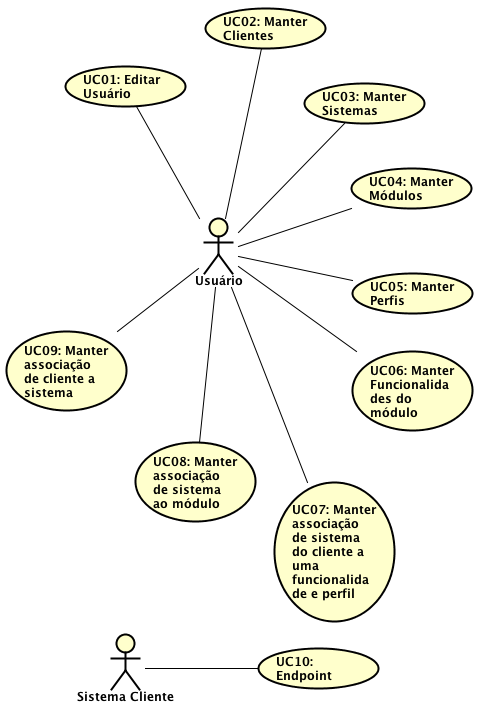
\includegraphics[width=1\textwidth]{img/Diagrama_de_caso_de_uso}
	\caption{Diagrama de caso de uso}
\end{figure}


Com a imagem \ref{fig:Diagrama de classe}, é possível compreender com mais clareza o funcionamento do back-end do software, visualizando as classes utilizadas para manipular os dados.

\begin{figure}
	\label{fig:Diagrama de classe}
	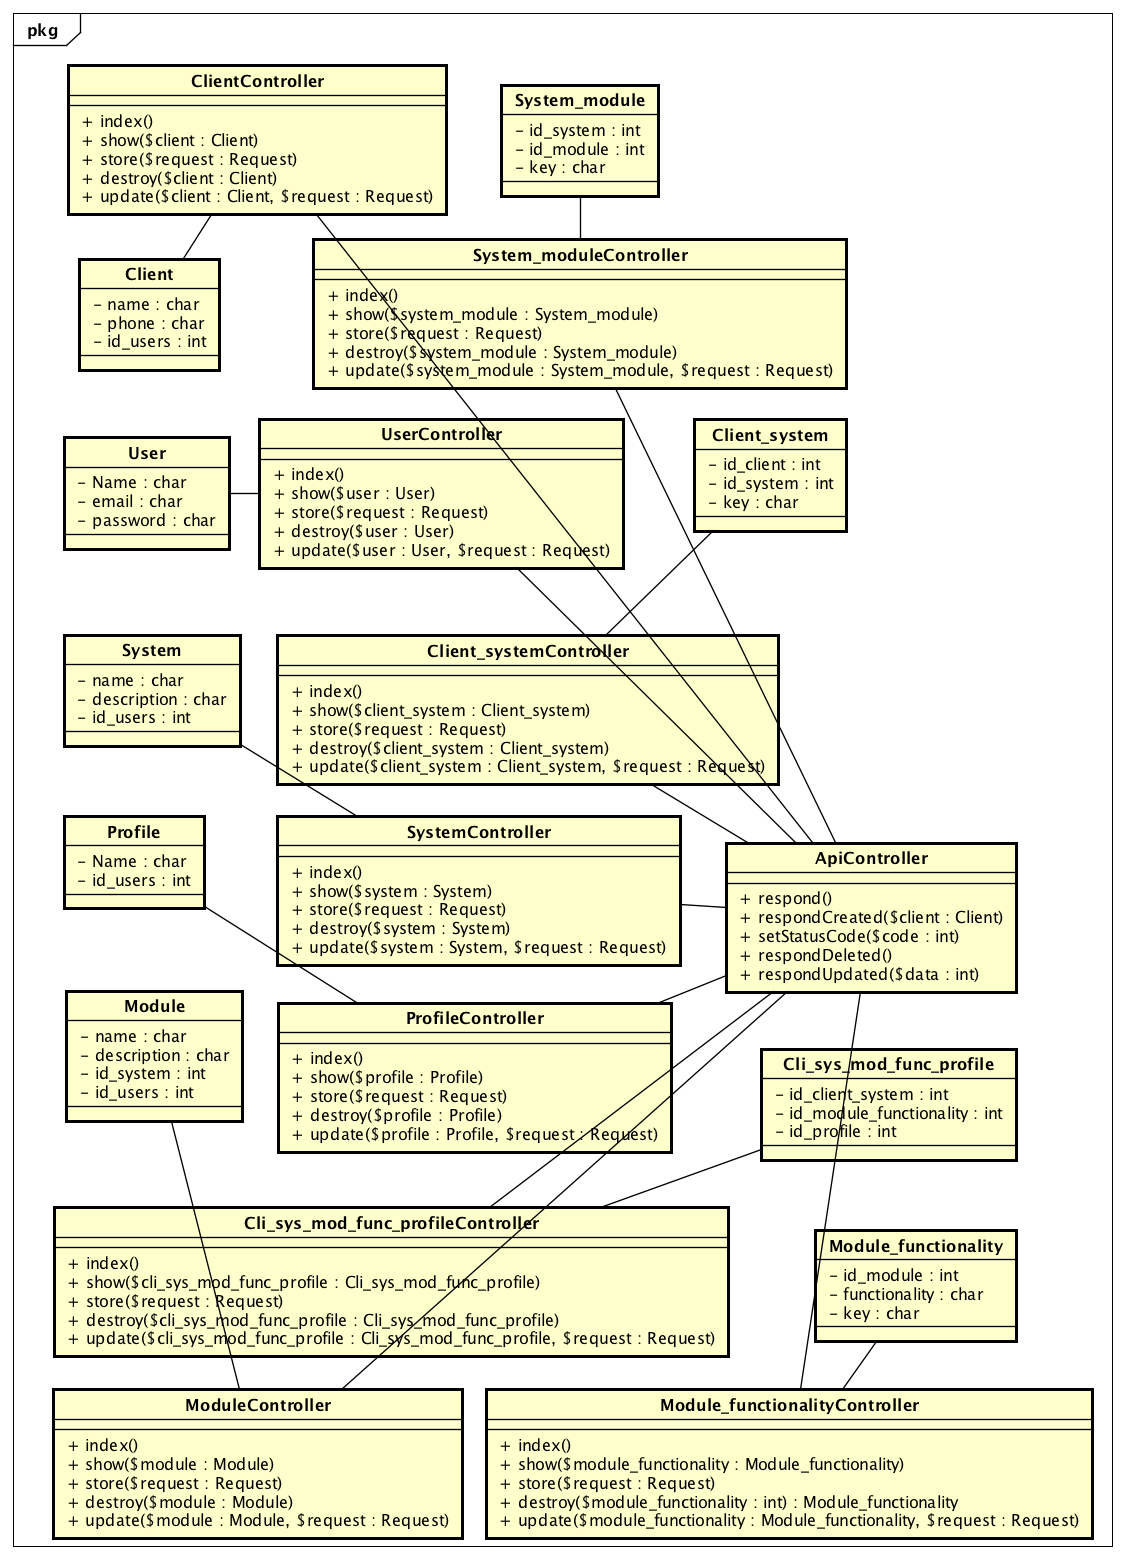
\includegraphics[width=1\textwidth]{img/Diagrama_de_classe}
	\caption{Diagrama de classe}
\end{figure}


Por fim, para prover um entendimento de funcionamento interno do software, a imagem \ref{fig:DER} traz o diagrama de entidade relacionamento, fornecendo uma ilustração da organização do banco de dados utilizado.


\begin{figure}
	\label{fig:DER}
	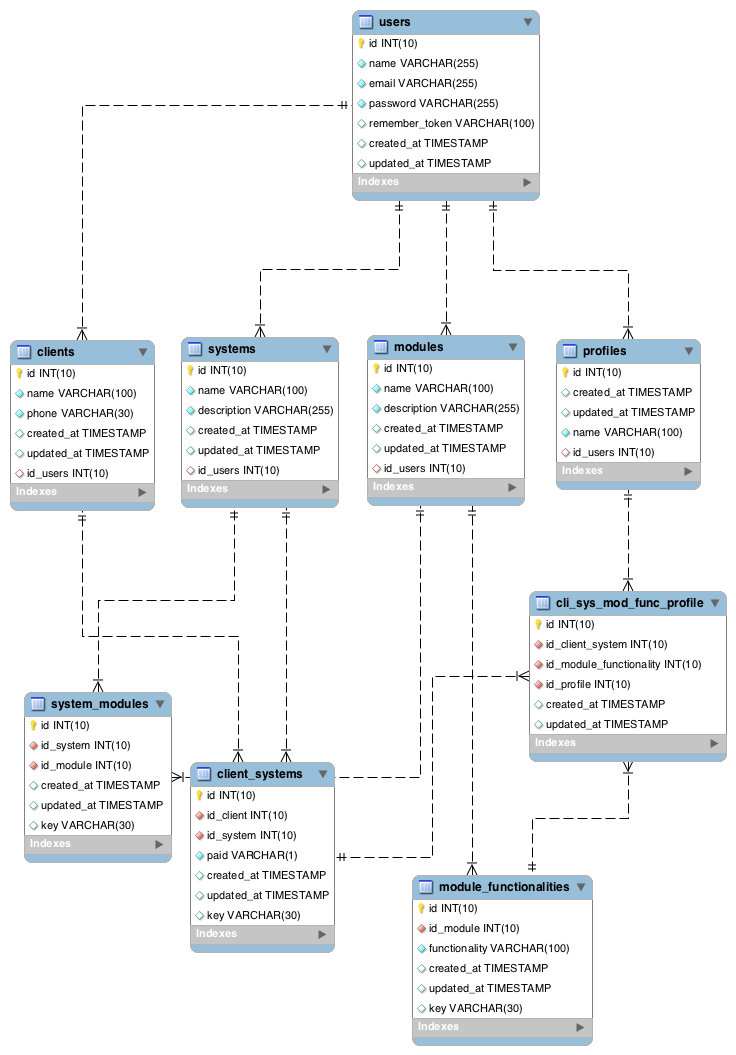
\includegraphics[width=1\textwidth]{img/DER}
	\caption{Diagrama entidade relacionamento}
\end{figure}


\subsection{Funcionalidades}\label{funcionalidades}

Esta seção apresenta os requisitos funcionais e não-funcionais implementados na aplicação proposta neste trabalho.


\subsubsection{Requisitos não funcionais}



\begin{itemize}
	
	
\item RN01: Usuários Simultâneos


Descrição: O sistema deverá suportar processamento multiusuário, ou seja, vários usuários poderão utilizar o sistema simultaneamente. 


\item RN02: Segurança 


Descrição: O sistema só permitirá acesso aos dados com autorização. Os usuários deverão se identificar usando um login e uma senha, e a referida senha será criptografada com a metodologia Bcrypt no banco de dados.


\item RN03: Alta disponibilidade 


Descrição: O sistema deverá ter disponibilidade de aproximadamente 99 porcento do tempo, a ser verificado com os logs do servidor.


\item RN04: Desempenho


Descrição: O tempo de resposta das consultas não deve ultrapassar 3 segundos, a ser validado com teste ao em produção.


\end{itemize}
	

\subsubsection{Requisitos funcionais}


\begin{itemize}
	
	
\item RF 01: Login


Descrição: O sistema deve conter tela de login com os campos email e senha. Após inserção dos dados, o sistema deve validar os dados e caso positivo, encaminhar o usuário ao sistema. Caso os dados sejam inválidos, exibir mensagem de erro para o usuário.


\item RF 02: Edição de usuário


Descrição: O sistema deve conter um formulário que seja carregado com os dados do usuário da sessão e permitir a atualização dos dados. Este requisito está relacionado ao UC01 da imagem \ref{fig:Diagrama de caso de uso}.


\item RF 03: Cadastro de cliente


Descrição: O sistema deve conter um formulário para cadastro de clientes. Após a inserção de um registro, o sistema deve automaticamente exibir o registro em formato de edição e conter botão para ir a uma consulta que liste os clientes cadastrados para o usuário da sessão. Este requisito está relacionado ao UC02 da imagem \ref{fig:Diagrama de caso de uso}.


\item RF 04: Cadastro de sistema


Descrição: O sistema deve conter um formulário para cadastro de sistemas. Após a inserção de um registro, o sistema deve automaticamente exibir o registro em formato de edição e conter botão para ir a uma consulta que liste os sistemas cadastrados para o usuário da sessão. Este requisito está relacionado ao UC03 da imagem \ref{fig:Diagrama de caso de uso}.


\item RF 05: Cadastro de módulo


Descrição: O sistema deve conter um formulário para cadastro de módulos. Após a inserção de um registro, o sistema deve automaticamente exibir o registro em formato de edição e conter botão para ir a uma consulta que liste os módulos cadastrados para o usuário da sessão. Este requisito está relacionado ao UC04 da imagem \ref{fig:Diagrama de caso de uso}.


\item RF 06: Cadastro de perfil


Descrição: O sistema deve conter um formulário para cadastro de perfil. Após a inserção de um registro, o sistema deve automaticamente exibir o registro em formato de edição e conter botão para ir a uma consulta que liste os perfils cadastrados para o usuário da sessão. Este requisito está relacionado ao UC05 da imagem \ref{fig:Diagrama de caso de uso}.


\item RF 07: Cadastro associativo de cliente aos sistemas


Descrição: O sistema deve conter um formulário para cadastro associativo de clientes a sistemas. Após a inserção de um registro, o sistema deve automaticamente gerar uma chave de acesso do dado registro para o usuário consultar permissões e exibir o registro em formato de edição e conter botão para ir a uma consulta que liste os registros associativos de clientes aos sistemas cadastrados para o usuário da sessão. Este requisito está relacionado ao UC09 da imagem \ref{fig:Diagrama de caso de uso}.


\item RF 08: Cadastro associativo de  sistemas aos módulos


Descrição: O sistema deve conter um formulário para cadastro associativo de sistemas a módulos. Após a inserção de um registro, o sistema deve automaticamente gerar uma chave de acesso do dado registro para o usuário consultar permissões e exibir o registro em formato de edição e conter botão para ir a uma consulta que liste os registros associativos de  sistemas aos módulos cadastrados para o usuário da sessão. Este requisito está relacionado ao UC08 da imagem \ref{fig:Diagrama de caso de uso}.


\item RF 09: Cadastro de funcionalidade dos módulos


Descrição: O sistema deve conter um formulário para cadastro de funcionalidade dos módulos já cadastrados. Após a inserção de um registro, o sistema deve automaticamente gerar uma chave de acesso do dado registro para o usuário consultar permissões e exibir o registro em formato de edição e conter botão para ir a uma consulta que liste os registros de funcionalidades cadastradas para o usuário da sessão. Este requisito está relacionado ao UC06 da imagem \ref{fig:Diagrama de caso de uso}.


\item RF 10: Composição de permissão para os módulos dos clientes


Descrição: O sistema deve conter um formulário para cadastro associativo de permissão para os módulos dos clientes. Após a inserção de um registro, o sistema deve automaticamente exibir o registro em formato de edição e conter botão para ir a uma consulta que liste os registros associativos de permissão cadastrados para o usuário da sessão. Este requisito está relacionado ao UC07 da imagem \ref{fig:Diagrama de caso de uso}.


\item RF 11: Endpoint


Descrição: O sistema deve disponibilizar uma URL para receber uma requisição via post, onde o deve receber um parâmetro "key", contendo a chave de acesso desejada para consultar as permissões cadastradas. Ao realizar a requisiçao enviando a "key", o sistema deve retornar um texto no formato Json, contendo os dados das permissões que foram compostas no sistema pelo usuário. A chave enviada pelo usuário pode ser de qualquer um dos níveis de configuração realizado no sistema e o o endpoint deve retornar a resposta sempre num mesmo formato, viabilizando um tratamento único da resposta pelo cliente. Este requisito está relacionado ao UC10 da imagem \ref{fig:Diagrama de caso de uso}.


\end{itemize}

\section{Processo}\label{sec:processo}


Para melhor compreensão do sistema proposto, a figura \ref{fig:diagramaBpmn} apresenta uma visão geral do processo implementado na ferramenta, utilizando, para tal, a notação BPMN.


\begin{figure} %\landscape 
	\vspace*{-2cm}
	\makebox[\linewidth]{
		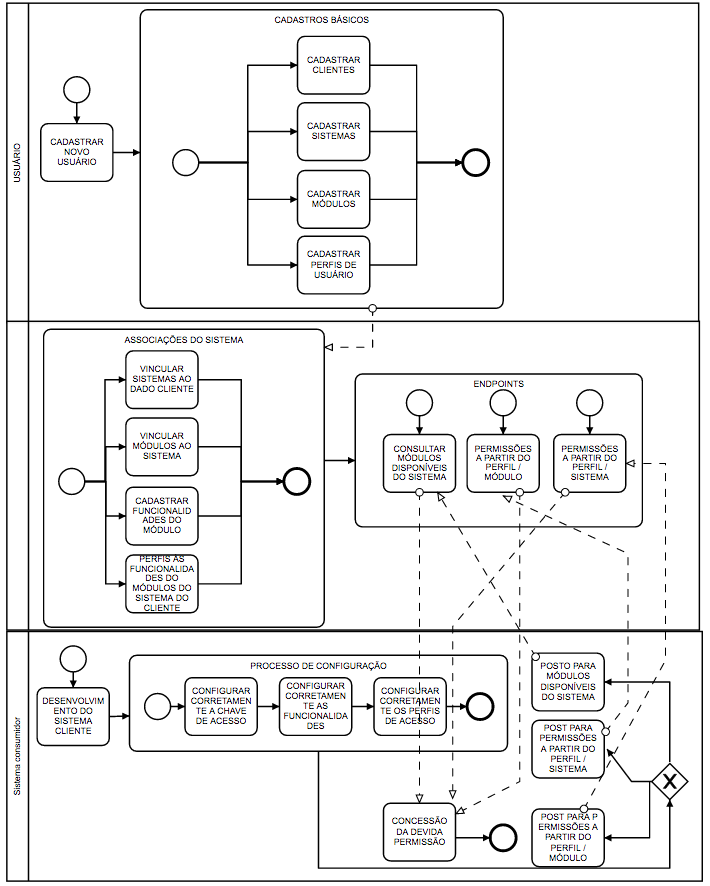
\includegraphics[width=1.3\linewidth]{img/diagrama_bpmn}
	}
	\label{fig:diagramaBpmn}
	\caption{Diagrama do processo(BPMN) do software em questão}
\end{figure}


\section{O que há de novo ?}\label{sec:novidades} %Sob o ponto de vista tecnológico


Seguindo a norma de padranização de código, com o software proposto é possível unificar o módulo de permissões de acesso e tratá-lo como um serviço, tornando possível eliminá-lo de qualquer software que faça uso do mesmo. A bordagem proposta neste trabalho de conclusão não é trivial, trata-se de uma aplicabilidade diferente do controle de permissão dos perfis, que não foi adotado por nenhum sistema disponível no estado da prática.